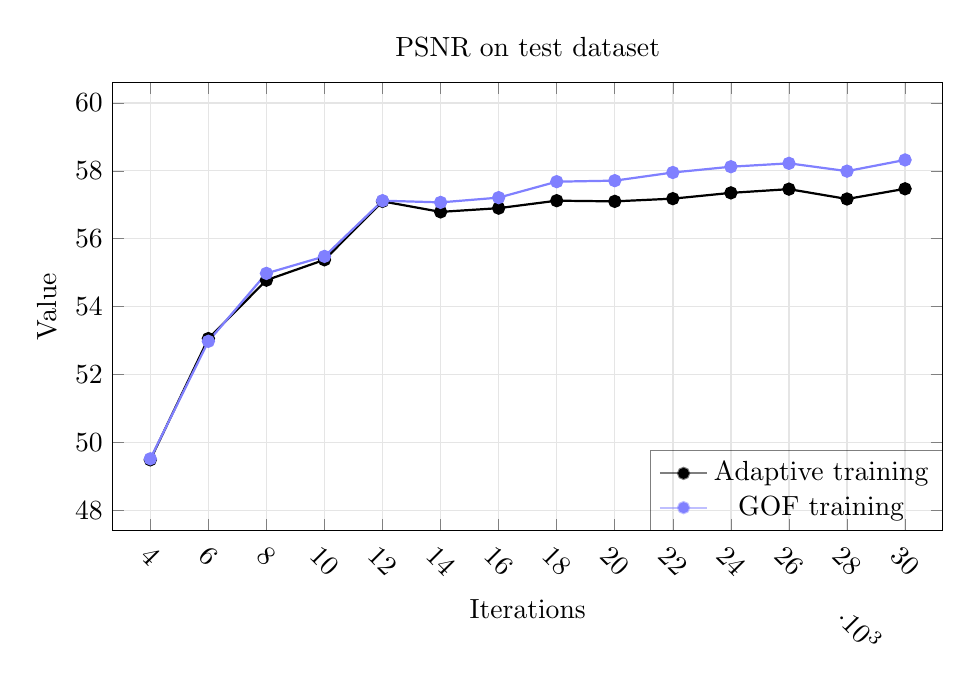
\begin{tikzpicture}
\begin{axis} [
title={PSNR on test dataset},
width=\linewidth,
height=0.6\linewidth,
axis lines= box,
xlabel near ticks,
ylabel near ticks,
xlabel={Iterations},
ylabel={Value},
xmin=4000,
xmax=30000,
ymin=48,
ymax=60,
xtick={4000,6000,...,30000},
ytick={48,50,...,60},
scaled x ticks={base 10:-3},
xticklabel style={rotate=315},
grid=major,
minor tick num=0,
grid style={line width=.1pt, draw=black!10},
major grid style={line width=.5pt,draw=black!10},
legend style={at={(1.0,0.0)},anchor=south east,fill=none,draw opacity=0.5},
enlargelimits=0.05,
]
\addplot[mark=*,thick] coordinates {
(4000,49.49)
(6000,53.06)
(8000,54.78)
(10000,55.38)
(12000,57.10)
(14000, 56.79)
(16000, 56.90)
(18000, 57.12)
(20000, 57.10)
(22000, 57.18)
(24000, 57.35)
(26000, 57.46)
(28000, 57.17)
(30000, 57.47)
};
\addlegendentry{Adaptive training}
\addplot[mark=*,thick,blue!50] coordinates {
(4000,49.52)
(6000,52.98)
(8000,54.98)
(10000,55.48)
(12000,57.12)
(14000, 57.07)
(16000, 57.21)
(18000, 57.68)
(20000, 57.71)
(22000, 57.95)
(24000, 58.12)
(26000, 58.22)
(28000, 57.99)
(30000, 58.32)
};
\addlegendentry{GOF training}
\end{axis}
\end{tikzpicture}
